% Options for packages loaded elsewhere
\PassOptionsToPackage{unicode}{hyperref}
\PassOptionsToPackage{hyphens}{url}
%
\documentclass[
  9pt,
  ignorenonframetext,
]{beamer}
\usepackage{pgfpages}
\setbeamertemplate{caption}[numbered]
\setbeamertemplate{caption label separator}{: }
\setbeamercolor{caption name}{fg=normal text.fg}
\beamertemplatenavigationsymbolsempty
% Prevent slide breaks in the middle of a paragraph
\widowpenalties 1 10000
\raggedbottom
\setbeamertemplate{part page}{
  \centering
  \begin{beamercolorbox}[sep=16pt,center]{part title}
    \usebeamerfont{part title}\insertpart\par
  \end{beamercolorbox}
}
\setbeamertemplate{section page}{
  \centering
  \begin{beamercolorbox}[sep=12pt,center]{part title}
    \usebeamerfont{section title}\insertsection\par
  \end{beamercolorbox}
}
\setbeamertemplate{subsection page}{
  \centering
  \begin{beamercolorbox}[sep=8pt,center]{part title}
    \usebeamerfont{subsection title}\insertsubsection\par
  \end{beamercolorbox}
}
\AtBeginPart{
  \frame{\partpage}
}
\AtBeginSection{
  \ifbibliography
  \else
    \frame{\sectionpage}
  \fi
}
\AtBeginSubsection{
  \frame{\subsectionpage}
}
\usepackage{lmodern}
\usepackage{amsmath}
\usepackage{ifxetex,ifluatex}
\ifnum 0\ifxetex 1\fi\ifluatex 1\fi=0 % if pdftex
  \usepackage[T1]{fontenc}
  \usepackage[utf8]{inputenc}
  \usepackage{textcomp} % provide euro and other symbols
  \usepackage{amssymb}
\else % if luatex or xetex
  \usepackage{unicode-math}
  \defaultfontfeatures{Scale=MatchLowercase}
  \defaultfontfeatures[\rmfamily]{Ligatures=TeX,Scale=1}
\fi
\usetheme[]{Goettingen}
\usecolortheme{rose}
% Use upquote if available, for straight quotes in verbatim environments
\IfFileExists{upquote.sty}{\usepackage{upquote}}{}
\IfFileExists{microtype.sty}{% use microtype if available
  \usepackage[]{microtype}
  \UseMicrotypeSet[protrusion]{basicmath} % disable protrusion for tt fonts
}{}
\makeatletter
\@ifundefined{KOMAClassName}{% if non-KOMA class
  \IfFileExists{parskip.sty}{%
    \usepackage{parskip}
  }{% else
    \setlength{\parindent}{0pt}
    \setlength{\parskip}{6pt plus 2pt minus 1pt}}
}{% if KOMA class
  \KOMAoptions{parskip=half}}
\makeatother
\usepackage{xcolor}
\IfFileExists{xurl.sty}{\usepackage{xurl}}{} % add URL line breaks if available
\IfFileExists{bookmark.sty}{\usepackage{bookmark}}{\usepackage{hyperref}}
\hypersetup{
  pdftitle={BIOS6643 Longitudinal},
  pdfauthor={EJC},
  hidelinks,
  pdfcreator={LaTeX via pandoc}}
\urlstyle{same} % disable monospaced font for URLs
\newif\ifbibliography
\setlength{\emergencystretch}{3em} % prevent overfull lines
\providecommand{\tightlist}{%
  \setlength{\itemsep}{0pt}\setlength{\parskip}{0pt}}
\setcounter{secnumdepth}{-\maxdimen} % remove section numbering
\AtBeginSubsection{}
\AtBeginSection{}
\ifluatex
  \usepackage{selnolig}  % disable illegal ligatures
\fi

\title{BIOS6643 Longitudinal}
\subtitle{L16 Gaussian Quadrature}
\author{EJC}
\date{}
\institute{Department of Biostatistics \& Informatics}

\begin{document}
\frame{\titlepage}

\begin{frame}[allowframebreaks]
  \tableofcontents[hideallsubsections]
\end{frame}
\hypertarget{gaussian-quadrature}{%
\section{Gaussian Quadrature}\label{gaussian-quadrature}}

\begin{frame}{Topics for today}
\protect\hypertarget{topics-for-today}{}
\begin{itemize}
\item
  Generalized linear mixed models (GzLMM)
\item
  Approximating the likelihood function associated with the GzLMM
\end{itemize}

\vspace{\baselineskip}

\begin{itemize}
\tightlist
\item
  \textbf{Related reading: Sections 5 in Non-normal notes.}
\end{itemize}
\end{frame}

\begin{frame}{Generalized linear mixed models (GzLMM)}
\protect\hypertarget{generalized-linear-mixed-models-gzlmm}{}
GzLMMs combine generalized linear model and linear mixed model theory.
There are greater complexities in fitting GzLMMs, due to nonlinearity
involved with the model.

When extending GzLM theory to longitudinal data, we consider the mean
link function in terms of both subject (\(i\)) and time (\(j\)):
\(g(\mu_{ij} )=\pmb {X_{ij}^r \beta}\), where \(\pmb X_{ij}^r\) denotes
the \(j\)th row of \(\pmb X_i\) (if considering the subject-specific
model) or the (\(ij\))th row of \(\pmb X\) (if considering the full data
model).

We could extend the model to other types of clustered data but for now
we'll just focus on longitudinal data.
\end{frame}

\begin{frame}{}
\protect\hypertarget{section}{}
Adding the `mixed' component, \(\pmb {Z_{ij}^r b_i}\), to the mean link
function for a longitudinal GzLM yields a GzLMM:
\(g(\mu_{ij} ) =\pmb {X_{ij}^r \beta}+\pmb {Z_{ij}^r b_i}\)

where \(g\) is a link as previously discussed (e.g., log link for
counts, logit link for binary outcomes),
\(\mu_{ij}=E[Y_{ij} |b_i,\ x_{ij}]\),
\(\pmb b_i \sim \mathcal N (\pmb 0,\ \pmb G_i)\), and \(\pmb Z_{ij}^r\)
is the \(j\)th row of \(\pmb Z_i\), the covariate matrix for subject
\(i\), associated with random effects \(\pmb b_i\).

The left side of a GzLMM looks like a GzLM and the right side looks much
like an LMM. The mean is often simplified to \(\mu_{ij}=E[Y_{ij} |b_i]\)
in the literature (or my notes), where conditioning on \(x_{ij}\) (and
parameters) is implied.

Interpretation of effects associated with GzLMMs are different than
those based on GzLM/GEEs, which will be discussed more later.

For a GzLMM, the linear predictor is generalized from the standard GzLM
by the addition of random effects:
\(\eta _{ij}=\pmb {X_{ij}^r \beta}+\pmb {Z_{ij}^r b_i}\).
\end{frame}

\begin{frame}{}
\protect\hypertarget{section-1}{}
We can express the model in `complete data' form as
\(g(\pmb \mu)= \pmb {X\beta} + \pmb {Zb}\), where
\(\pmb \mu =E[\pmb Y|\pmb b,\ \pmb x]\) (an \(r_{tot} \times 1\) vector)
and quantities on the right-hand side of the equation are defined as in
the early part of the LMM notes. An expression of the model above that
will be useful for estimation discussed later is
\(\pmb \mu = g^{-1} (\pmb {X\beta} + \pmb {Zb})\).

Fitting of the GzLMMs does not involve GEE. Two common approaches used
include approximating the true likelihood function or using
pseudo-likelihood estimation; we'll talk about the former today.
\end{frame}

\begin{frame}{Fitting the GzLMM by approximating the likelihood
function}
\protect\hypertarget{fitting-the-gzlmm-by-approximating-the-likelihood-function}{}
Let \(h(\pmb b_i)\) and \(f(y_i)\) denote the pdf's of the random
effects and responses for subject \(i\), respectively. Also, let
\(l(y_i | \pmb b_i)\) denote the conditional pdf of of the responses
given the random effects that is a member of the exponential family
(e.g., Poisson, binomial, geometric, gamma). Then, we can express the
density of the responses as
\(f(\pmb y_i) = \int l(\pmb y_i |\pmb b_i)h(\pmb b_i)d\pmb b_i\) for
subjects \(i=1,\ ...,\ n\). This will be useful in setting up a
likelihood equation for estimation of parameters.

When subjects are assumed to be independent (the standard case), then
the likelihood function is \(L=\prod _{i=1}^nf(\pmb y_i)\). For
computation we can use \(ln(L)=\sum _{i=1}^nln[f(\pmb y_i)]\).
\end{frame}

\begin{frame}{}
\protect\hypertarget{section-2}{}
For normal outcomes, the likelihood could be expressed in closed form
because the integral in the likelihood function involves only normal
distributions, but numerical techniques were required to optimize the
function. For non-normal outcomes, the function cannot even be written
in closed form.

However, we can approximate the log-likelihood function using a
numerical integration technique such as Gaussian quadrature. In this
case our original likelihood,
\(L=\prod _{i=1}^n\int l(\pmb y_i |\pmb b_i)h(\pmb b_i)d\pmb b_i\) is
approximated as
\(L\approx \prod _{i=1}^n\sum _{k=1}^Kl(\pmb y_i |\pmb b_i=\pmb v_k)w_k\)
where \(K\) is the number of quadrature points, vk are evaluation points
(or abscissae, or nodes) and wk are weights. The weights and evaluation
points are chosen to optimize the approximation. {[}See Fitzmaurice et
al.~for more detail.{]}

An optimization technique such as the Dual Quasi-Newton method can then
be be used to maximize the approximate function in order to determine
maximum likelihood parameter estimates.

As with standard LMM's, the random effects can then be estimated as the
mean of the random effects distribution, given the data and parameter
estimates.
\end{frame}

\begin{frame}{Software to fit GzLMMs using Gaussian quadrature}
\protect\hypertarget{software-to-fit-gzlmms-using-gaussian-quadrature}{}
SAS has two procedures available to approximate a GzLMM using adaptive
Gaussian quadrature, after which a dual Quasi-Newton method is used to
optimize the function:

\begin{itemize}
\item
  PROC NLMIXED
\item
  PROC GLIMMIX: specify \emph{method=quad} to perform adaptive Gaussian
  quadrature or \emph{method=laplace} to use Laplace's method (the
  latter is equivalent to \emph{method=quad} with 1 quadrature point).
\end{itemize}

In R, the \textbf{glmer()} function in the \textbf{lme4} package can be
used to approximate a GzLMM using Gaussian quadrature.

SAS uses \emph{adaptive} quadrature by default, meaning the number of
quadrature points is selected based on the data, model and specified
tolerance limits. But with both SAS and R, the number of quadrature
points can also be specified.
\end{frame}

\begin{frame}{}
\protect\hypertarget{section-3}{}
SAS and R use Gauss-Hermite quadrature (a specific type of Gaussian
quadrature) to fit likelihoods for GzLMM's, which accounts for the
\(exp⁡(-b_i^2\)) term in the density of random effects (part of the
normal density); this term becomes part of the weights (will illustrate
later).

To demonstrate the different procedures, exacerbation data from the
Kunsberg kids / air pollution study was used. In this case, the 2003-04
study year was used; otherwise data are similar to that presented in the
`Non-normal' notes. The code and abbreviated output follow, using 7
quadrature points.

\begin{center}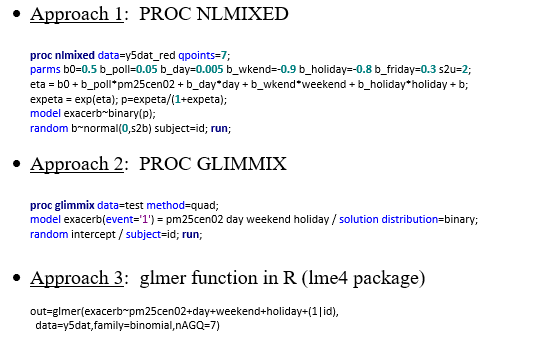
\includegraphics[width=0.7\linewidth]{figs_L15/f1} \end{center}
\end{frame}

\hypertarget{some-notes}{%
\section{Some notes}\label{some-notes}}

\begin{frame}{Some notes:}
\protect\hypertarget{some-notes-1}{}
Data below use 6923 observations on 43 subjects. The outcome is
exacerbation (1=yes, 0=no); logit link.

In SAS PROC GLIMMIX the number of quadrature points (7) was selected
adaptively based on the data and model at hand, and the default
tolerance limit; in R we requested it using the nAGQ argument and with
PROC NLMIXED we obtained it using an option. If no nAGQ option is given,
R will use 1 quadrature point (i.e., Laplace method).

From SAS Documentation: ``The quadrature rule in the GLIMMIX procedure
is adaptive in the following sense: if you do not specify the number of
quadrature points with the QPOINTS= suboption of the METHOD=QUAD option,
then the number of quadrature points is determined by evaluating the log
likelihood at the starting values at a successively larger number of
nodes until a tolerance is met.''
\end{frame}

\begin{frame}{}
\protect\hypertarget{section-4}{}
NLMIXED also uses an adaptive approach by default, although you might
end up with different number of quadrature points compared with GLIMMIX.
For example, to get 7 quadrature points for the data above in NLMIXED
without specifying the QPOINTS option, I need to change QTOL from
\(10^{-4}\) to \(10^{-5}\): proc nlmixed data=y5dat qtol=0.00001;. I
believe the default QTOL is the same in GLIMMIX, but they may have
different meanings based on how data are processed by the different sets
of code.

R also stats that the quadrature is adaptive, although I am not sure in
what sense. Their documentation states that the number of quadrature
points defaults to 1, in which case it does say it is using Laplace
approximation; to get more than 1 point, you need to specify it, in
which case it says `Adaptive' quadrature is used, but to get this, the
number of points is specified!
\end{frame}

\begin{frame}{Abbreviated output for the 3 approaches}
\protect\hypertarget{abbreviated-output-for-the-3-approaches}{}
\begin{center}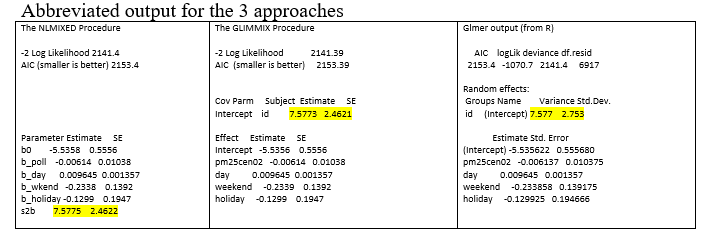
\includegraphics[width=0.7\linewidth]{figs_L15/f2} \end{center}

The results are quite similar, except for the higher SE for the subject
variance estimate.

In addition, the GLIMMIX code (Approach 2, middle), displays fit
statistics for the conditional distribution:

Fit Statistics for Conditional Dist.

-2 log L(exacerb \textbar{} r. effects): 1995.76 Pearson Chi-Square:
4398.25 Pearson Chi-Square / DF: 0.64
\end{frame}

\begin{frame}{}
\protect\hypertarget{section-5}{}
The level of accuracy of estimates is controlled by the number of
quadrature points used in the approximation. You can specify this in the
method option.

When the number of quadrature points is 1, Gaussian quadrature is
equivalent to Laplace's method. The following 3 statements can be used
to obtain Laplace's method.

\begin{center}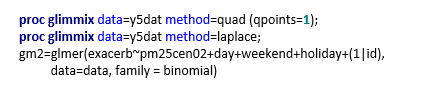
\includegraphics[width=0.7\linewidth]{figs_L15/f3} \end{center}

You need to consider the best number of quadrature points to use. The
more, the better, although as you increase it, the computational burden
increases. If \(K\) is the number of quadrature points and \(q\) is the
number of random effects (for each subjects), then ``the GLIMMIX
procedure evaluates \(K^q\) conditional log likelihoods for each
observation to compute one value of the objective function.'' (From SAS
Documentation.)
\end{frame}

\begin{frame}{}
\protect\hypertarget{section-6}{}
One possible approach would be to run GLIMMIX will default settings, and
then possibly increase the number of quadrature points incrementally and
see what impact it has on accuracy of the fit. The following shows
differences for our data when using 1 versus 7 quadrature points when
using PROC GLIMMIX.

\begin{center}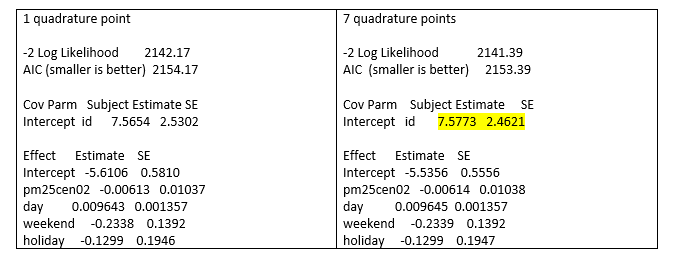
\includegraphics[width=0.7\linewidth]{figs_L15/f4} \end{center}
\end{frame}

\begin{frame}{Deriving the likelihood for GzLMM's}
\protect\hypertarget{deriving-the-likelihood-for-gzlmms}{}
Let \(h(\pmb b_i)\) and \(f(\pmb y_i)\) denote the pdf's of the random
effects and responses for subject \(i\), respectively. Also, let
\(l(\pmb y_i | \pmb b_i)\) denote the conditional pdf of the responses
given the random effects that is a member of the exponential family
(e.g., Poisson, binomial, geometric, gamma). Then, we can express the
density of the responses as
\(f(\pmb y_i)=\int l(\pmb y_i |\pmb b_i)h(\pmb b_i)d \pmb b_i\) for
subjects \(i=1,\ ...,\ n\). This will be useful in setting up a
likelihood equation for estimation of parameters.

When subjects are assumed to be independent (the standard case), then
the likelihood function is \(L=\prod _{i=1}^n f(\pmb y_i)\).
\end{frame}

\begin{frame}{}
\protect\hypertarget{section-7}{}
Let's consider the likelihood function for the GzLMM that has a binary
outcome and a random intercept for subjects. Specifically, let's
consider the following model

\(Y_{ij} |b_i \sim \mathcal {Bernoulli}(p_{ij})\), for \(i=1,\ ...,\ n\)
and \(j=1,\ ...,\ r\) \(ln[p_{ij}/(1-p_{ij})]=\beta x_{ij}+b_i\),
\(b_i \sim \mathcal N (0,\ \sigma ^2)\)

Note that
\(p_{ij}=P(Y_{ij}=1|b_i)=\frac {exp( b_i+\beta x_{ij})} { 1+exp( b_i+\beta x_{ij})}\)

(For the following, conditioning on covariates and parameters is
suppressed for convenience.) This is essentially taken from
\textbf{McCulloch's An Introduction to Generalized Linear Mixed Models}.
I am starting with the `data wide' model, where subjects are stacked
into the \(Y\) matrix (next page):
\end{frame}

\begin{frame}{}
\protect\hypertarget{section-8}{}
\[
L(\beta,\ \sigma ^2;\ \pmb y)=f(\pmb y)=\int l(\pmb y|\pmb b)h(\pmb b)d\pmb b \]

\vspace{-5mm}

\[ =\int_{\pmb b} P(\pmb Y= \pmb y| \pmb b)h(\pmb b)d\pmb b 
\]

\vspace{-5mm}

\[ 
=\int_{\pmb b}  \prod_{i, j} P(Y_{ij}=y_{ij} |b)h(b)db
\]

\vspace{-5mm}

\[ 
=\prod_i \int_{b_i}\prod_j P(Y_{ij}=y_{ij} |b_i)h(b_i)db_i
\]

Note that for \(y_{ij}=1\), we have
\(P(Y_{ij}=y_{ij} |b_i)=P(Y_{ij}=1|b_i)=p_{ij}\) and for \(y_{ij}=0\) we
have
\(P(Y_{ij}=y_{ij} |b_i)=P(Y_{ij}=0|b_i)=\frac 1 {1 + exp( b_i+\beta x_{ij})}\),
so collectively we can write
\(P(Y_{ij}=y_{ij} |b_i)= \frac {exp\big(y_{ij} (b_i+\beta x_{ij}) \big)} {1+exp(b_i+\beta x_{ij})}\).

Hence we can write

\[
L(\beta,\ \sigma ^2;\ \pmb y) = \prod_i \int_{b_i}\prod_j P(Y_{ij}=y_{ij} |b_i)h(b_i)db_i   =\prod_i \int{b_i}\prod_j \Bigg[ \frac {e^{y_{ij} (b_i+\beta x_{ij})}} {1+e^{b_i+\beta x_{ij}}} \Bigg] h(b_i) db_i 
\]

\vspace{-5mm}

\[
=\prod_i \int_{b_i} \prod_j \Bigg[\frac {e^{y_{ij} (b_i+\beta x_{ij})}} {1+e^{b_i+\beta x_{ij}}}\Bigg] \times \frac {e^{-b_i^2/2\sigma ^2}} {\sqrt{2\pi \sigma ^2 }} db_i  
\]

\vspace{-5mm}

\[
=\prod_i \int_{b_i} \frac {e^{\sum_j y_{ij} (b_i+\beta x_{ij})} } {\prod_j (1+e^{b_i+\beta x_{ij}})} \times \frac {e^{-b_i^2/2\sigma ^2}} {\sqrt{2\pi \sigma ^2 }} db_i
\]
\end{frame}

\begin{frame}{}
\protect\hypertarget{section-9}{}
We could also express the likelihood in a slightly more succinct form in
terms of the \(p_{ij}\) (e.g., see Parzen 2011):
\(L(\beta,\ \sigma ^2;\ \pmb y)=\prod_i \int _{b_i} \Big[ \prod_j p_{ij}^{y_{ij}} (1-p_{ij} )^{(1-y_{ij})} \times \frac {e^{-b_i^2/2\sigma ^2}} {\sqrt{2\pi \sigma ^2 }} \Big] db_i\)

Note that in order to maximize the likelihood we input the data (\(x\)
and \(y\) values). For example, say that one subject has 5 observed
\(y\) values of \((0,\  1,\ 1,\ 0,\ 1)\), with associated \(x\) values
of \((1,\ 2,\ 3,\ 4,\ 5)\). Then on the interior of the likelihood that
is within the square brackets on the last equation (for that subject
`\(i\)'), we would have (next page):
\end{frame}

\begin{frame}{}
\protect\hypertarget{section-10}{}
\[
(1-p_{i1})p_{i2} p_{i3} (1-p_{i4})p_{i5} \frac {e^{-b_i^2/2\sigma ^2}} {\sqrt{2\pi \sigma ^2 }} 
\]

\vspace{-5mm}

\[
 =\frac {e^{3b_i+10} e^{-b_i^2/2\sigma^2}} {\sqrt {2\pi \sigma ^2} \prod_j (1+e^{b_i+\beta_j})} 
 \]

\vspace{-5mm}

\[ =\frac {e^{3b_i+10-b_i^2/2\sigma ^2}}  {\sqrt {2\pi \sigma ^2 } (1+e^{b_i+\beta})(1+e^{b_i+2\beta})(1+e^{b_i+3\beta})(1+e^{b_i+4\beta})(1+e^{b_i+5\beta})}
\]

Note that we integrate over the last quantity with respect to \(b_i\),
then repeat for all subjects and multiply together. This gives a flavor
of the complexity of the integration. (Actual optimization uses the log
likelihood, in which case it is a matter of summing logged quantities
over subjects.)
\end{frame}

\hypertarget{illustration}{%
\section{Illustration}\label{illustration}}

\begin{frame}{Illustration of Gauss-Hermite quadrature}
\protect\hypertarget{illustration-of-gauss-hermite-quadrature}{}
Consider integration of the form
\(\int_{-\infty }^\infty e^{-x^2} f(x)dx\). Using Gauss-Hermite
quadrature we can approximate this quantity as
\(\sum _{i=1}^nw_i f(x_i)\), where \(w_i\) are weights used in place of
\(e^{-x^2}\).

As an illustration, consider \(X \sim \mathcal N (\mu,\ \sigma ^2)\) and
we wish to evaluate
\(E[f(X)] = \int_{-\infty }^\infty \frac 1 {\sigma \sqrt {2\pi}} e^{-\frac {(x-\mu)^2} {2\sigma ^2}} f(x) dx\).

Using a change of variables \(z=(x-\mu)/(\sqrt {2} \sigma )\) we can
perform integration by substitution to express
\(E[f(X)]=\int_{-\infty }^\infty 1/\sqrt {\pi} e^{-z^2} f(\sqrt {2} \sigma z+\mu) dz\).

Using this form we can then use the Gauss-Hermite rule to obtain
\(E[f(X)] \approx \frac 1 {\sqrt {\pi}} \sum _{i=1}^m w_i f(\sqrt {2} \sigma z_i+\mu)\).

The \(m\) (standardized) evaluation points, \(z_i\), \(i=1,\ ...,\ m\),
are the roots of the Hermite polynomial Hn(z), with weights
\(w_i=\frac {2^{n-1} m!\sqrt {\pi}} {m^2 [H_{m-1} (x_i)]^2}\)

In the approximation above, the weight variable takes the place of the
\(e^{-z^2}\) term.
\end{frame}

\begin{frame}{}
\protect\hypertarget{section-11}{}
For example, for \(m=5\), \(H_5 (z)= 32 z^5-160z^3+120z\) and
\(H_4(z)=16z^4-48z^2+12\), which yields
\(z_i=(-2.02, -0.96, 0, 0.96, 2.02)\) and
\(w_i=(0.02, 0.39, 0.95, 0.39, 0.02)\).

Notes: (i) the `roots' are the values of \(z\) that satisfy
\(H_5(z)=0\); (ii) more places can be kept for greater accuracy in the
actual calculation; (iii) more evaluation points can be used if greater
approximation for the numerical integration is required.

By setting the \(f(x)\) function to 1 we can use the Gauss-Hermite
approximation for the area under the curve itself:
\(\int_{-\infty }^\infty \frac 1 {\sigma \sqrt {2}\pi} e^{- \frac {(x-\mu)^2} {2\sigma ^2 }} dx= \frac 1 {\sqrt {\pi}} \int_{-\infty }^\infty e^{-z^2} dz=\frac 1 {\sqrt {\pi}} \sum _{i=1}^mw_i =1\).
I.e., the weights above sum up to the square root of \(\pi\).
\end{frame}

\begin{frame}{}
\protect\hypertarget{section-12}{}
The lower left graph shows the standard normal pdf, with the evaluation
points (x-axis) and weights (y-axis) used in the Gauss-Hermite
approximation approach using 5 evaluation points with the example above.
The curve is continuous and the numerical approximation uses discrete
points, but you could consider a histogram approximation by making a bar
for each discrete point that has width=1, and centered on the points,
shown on the right. The area of the histogram is 1, just like the area
under the curve, although individual bars may seem to be too high or
low.

\begin{center}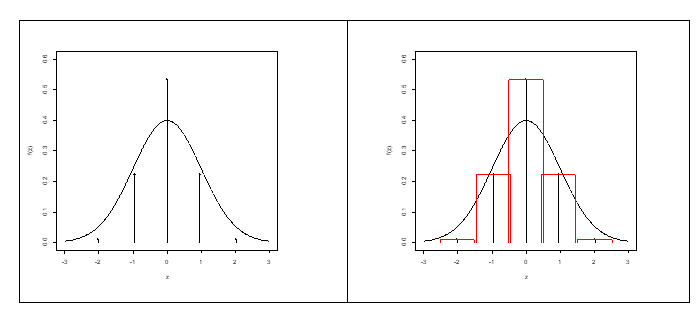
\includegraphics[width=0.7\linewidth]{figs_L15/f5} \end{center}
\end{frame}

\begin{frame}{}
\protect\hypertarget{section-13}{}
For another example, say \(f(X)=X^2,\ \mu=10\) and \(\sigma =2\). Using
the Gauss-Hermite approximation we find that \(E[X^2]=104\). We can
verify this quickly by employing the fact that
\(\Big(\frac {(X–10)} 2\Big)^2\) has a chi-square distribution with 1
degree of freedom.

These examples are simpler than Gauss-Hermite quadrature used for
approximating likelihoods of GzLMM's, which involve multiple subjects
and more complicated functions (e.g., the logistic likelihood previously
derived). However, the principle is the same.

Interpretation
\end{frame}

\begin{frame}{Interpreting random effects and associated covariance
parameters in GzLMM's}
\protect\hypertarget{interpreting-random-effects-and-associated-covariance-parameters-in-gzlmms}{}
For mixed models with non-normal outcomes, how do we interpret the
random effects and their covariance parameters?

It's pretty easy for normal models. For example, if we have a simple
random intercept LMM (plus fixed effects), a value of \(b_i=1.5\) means
that this subject is estimated to be 1.5 units higher than the average
value of Y. But for a logistic regression model, the same \(b_i\) value
would represent an increase in the log odds of 1.5, which relates to an
increase in odds of \(e^{1.5}=4.5\).

The same random effect value in a Poisson model with log link would
relate to a 4.5 times increase in outcome.
\end{frame}

\begin{frame}{}
\protect\hypertarget{section-14}{}
We could also put it in terms of probability by noting that
\(p_{ij}=P(Y_{ij}=1|b_i)=\frac {exp(b_i+\pmb {X_{ij}^r \beta})} {1+exp( b_i+\pmb {X_{ij}^r \beta})}\)
and then compare \(p_{ij}\) for \(b_i=0\) vs.~that of \(b_i=1.5\).
Unfortunately, this comparison depends on values of predictors unless
there is only a fixed intercept in the model.

To interpret covariance parameters, we also need to consider the link
used. Consider again the logistic regression model with a random
intercept: \(ln⁡[ p_{ij}/(1-p_{ij})]=\pmb {X_{ij}^r \beta}+b_i\), where
\(b_i \sim \mathcal N (0,\sigma_b^2)\). If \(\sigma_b^2=2\), then the
standard deviation of the distribution of \(ln (p_{ij}/(1-p_{ij} ))\)
(given \(\pmb X_{ij}^r\) and \(\pmb \beta\)) is 1.4.

We also note that
\(p_{ij}/(1-p_{ij})=exp(\pmb {X_{ij}^r \beta}+b_i)=exp(\pmb {X_{ij}^r \beta})exp(b_i)\).
As exp(b\_i) has a log-Normal distribution with variance
\(exp(2\sigma_b^2 )-exp(\sigma_b^2)\), it follows that the variance of
the odds is
\(Var[p_{ij}/(1-p_{ij})]=[exp(\pmb {X_{ij}^r \beta})]^2 Var[exp(b_i)] =[exp(\pmb {X_{ij}^r \beta})]^2 [exp(2\sigma_b^2 )-exp(\sigma_b^2 )]\).
But this may be harder to interpret it as the odds has a skewed
distribution.
\end{frame}

\hypertarget{precision}{%
\section{Precision}\label{precision}}

\begin{frame}{Estimating precision}
\protect\hypertarget{estimating-precision}{}
Variance and covariance estimators associated with parameter estimators
in the GzLMM can be derived from the inverse of the negative Hessian
matrix.

For more detail on this, as well as a description of covariances that
include random effect terms as well as fixed-effect estimators (i.e.,
\(Var[(\pmb {\hat \beta}, \pmb {\hat b})^{\top}]\)), see the SAS Help
Documentation under PROC GLIMMIX, Details, Aspects Common to Adaptive
Quadrature and Laplace Approximation.
\end{frame}

\hypertarget{summary}{%
\section{Summary}\label{summary}}

\begin{frame}{Summary}
\protect\hypertarget{summary-1}{}
\end{frame}

\end{document}
